\documentclass[12pt,a4paper,oneside]{article}
\usepackage[colorlinks=true,unicode]{hyperref}
\usepackage[utf8]{inputenc}
\usepackage[czech]{babel}
\usepackage{graphicx}
\usepackage{pdfpages}
\textwidth 16cm \textheight 25cm
\topmargin -1.3cm 
\oddsidemargin 0cm
\usepackage{footnote}
\pagestyle{empty}
\begin{document}
\title{Převodník logiky TTL na PECL TTLPECL01A}
\author{Jakub Kákona, kaklik@mlab.cz}
\maketitle

\thispagestyle{empty}
\begin{abstract}
Modul je jednosměrným translátorem mezi logickými úrovněmi
PECLa TTL. Směr převodu je vybrán během osazení modulu zvoleným typem obvodu
\end{abstract}

\begin{figure} [htbp]
\begin{center}
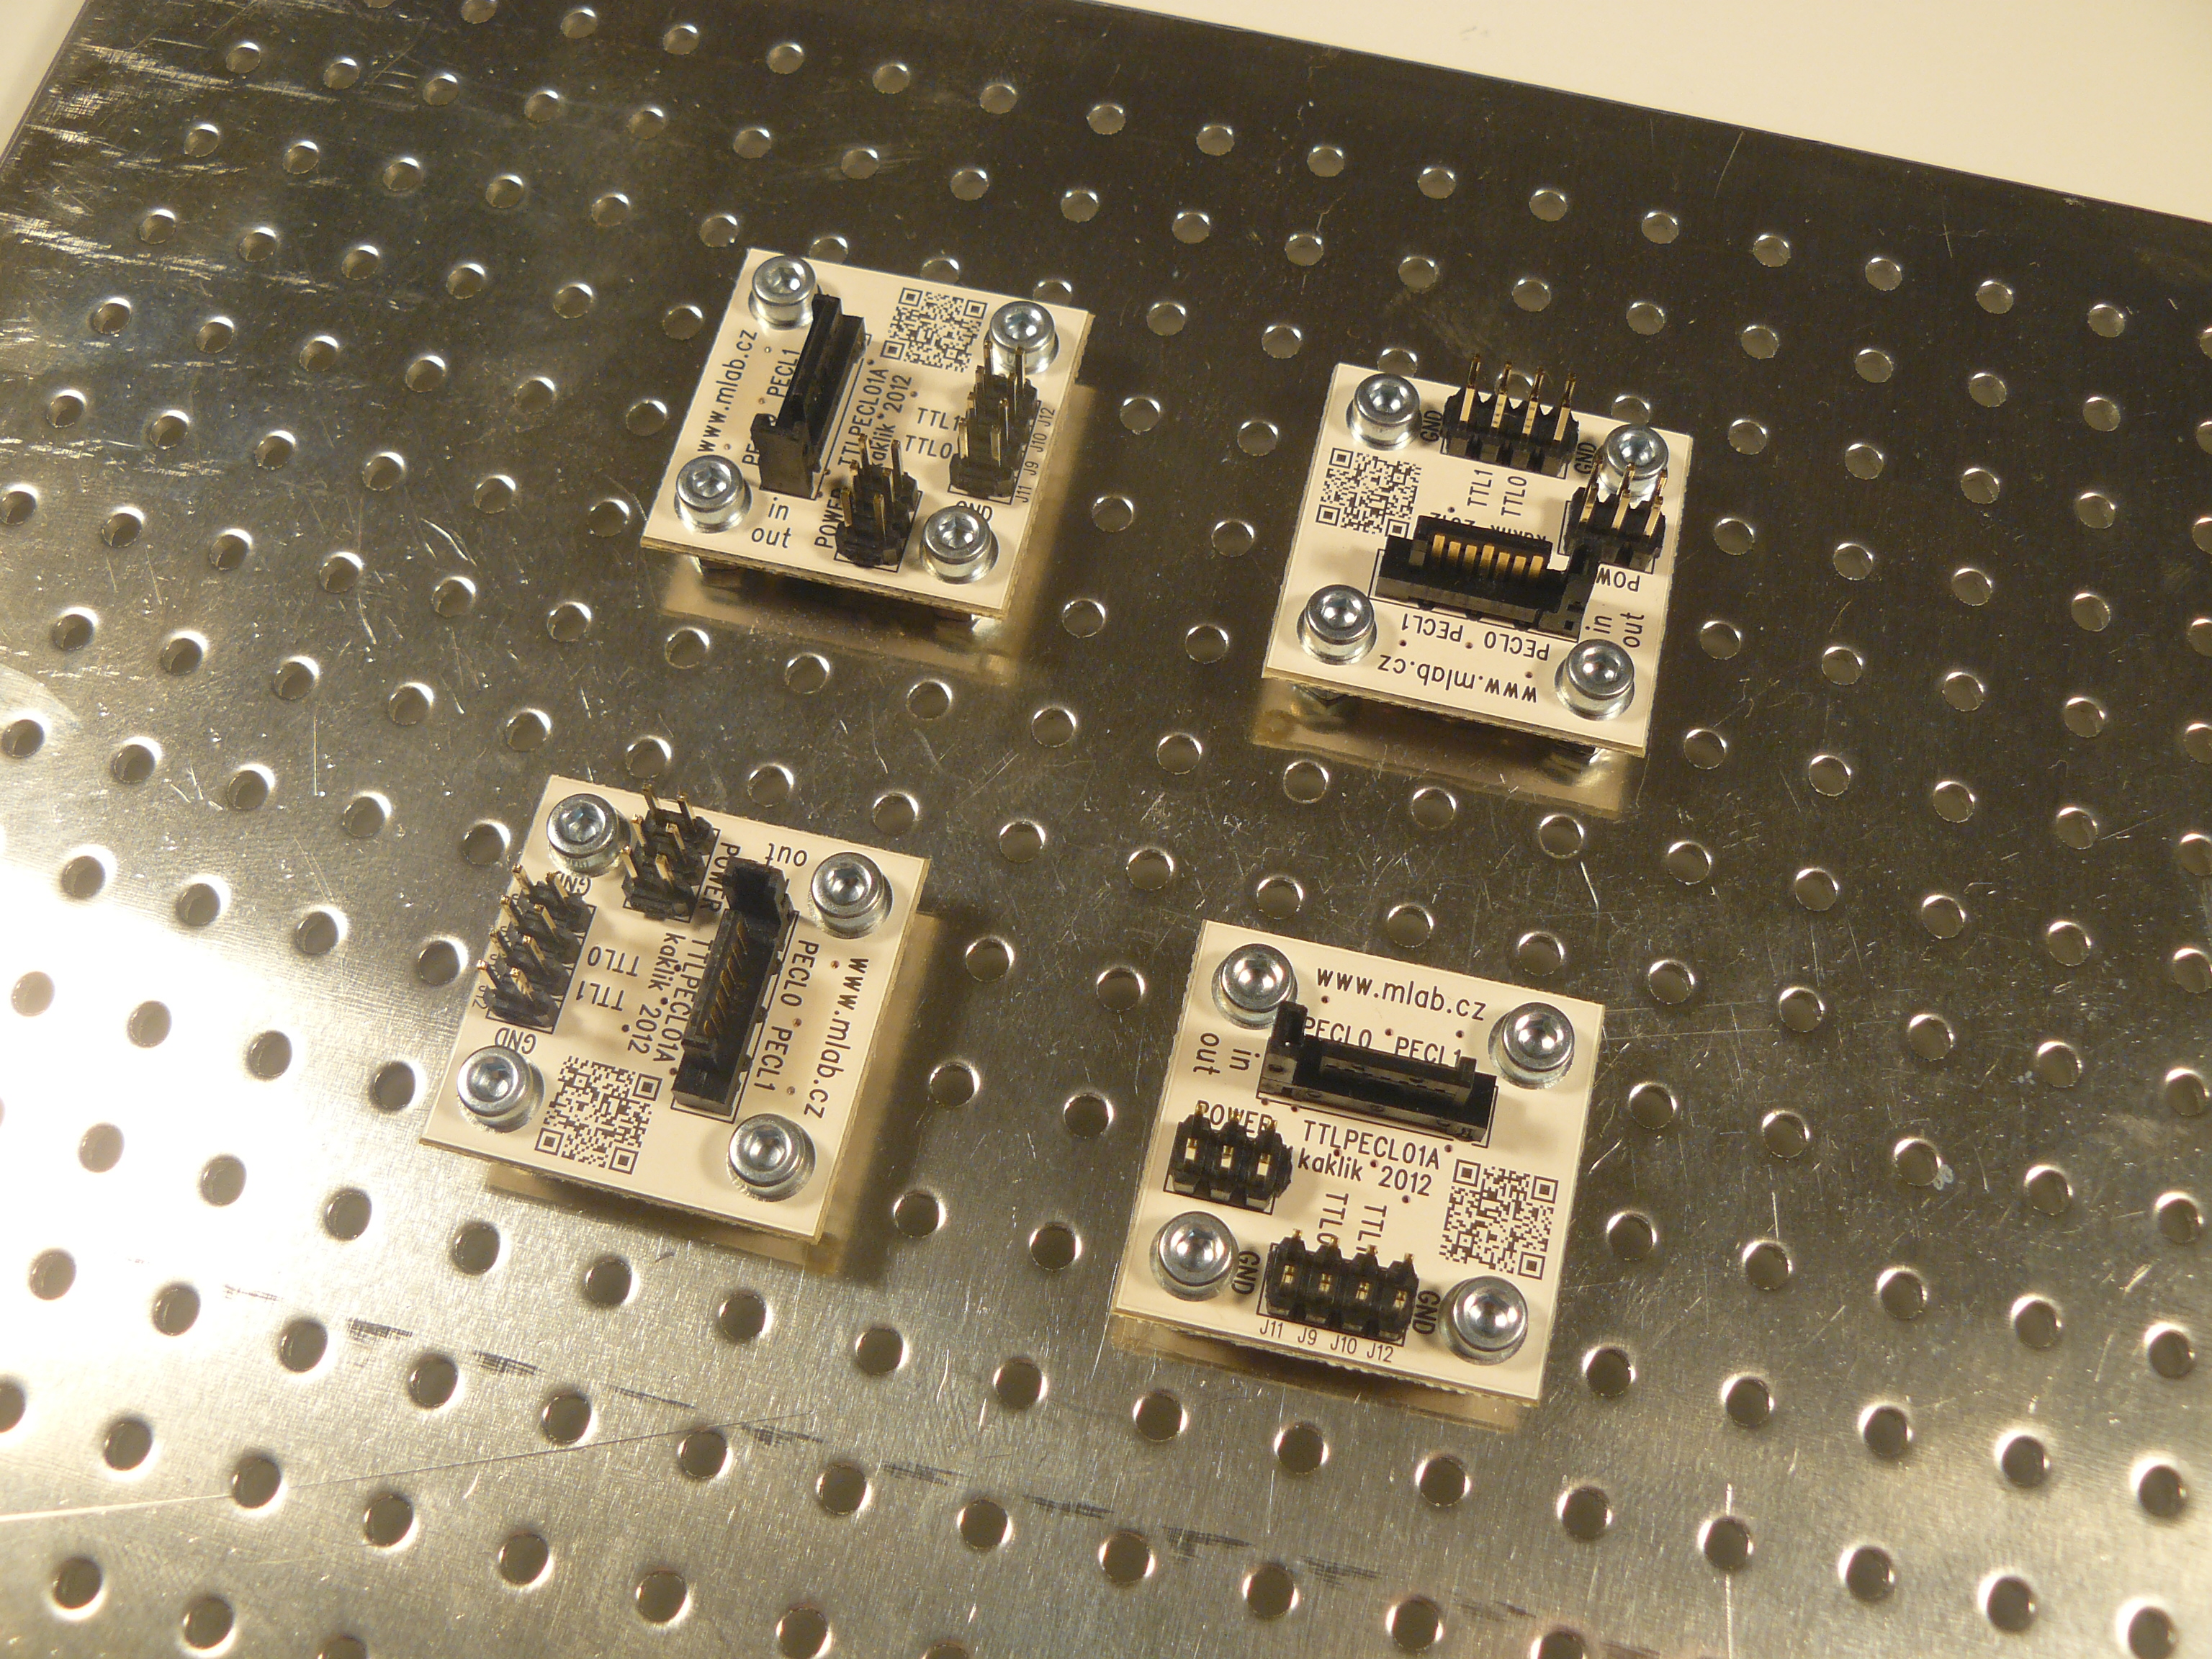
\includegraphics [width=80mm] {./img/TTLPECL01A_Top_Big.JPG} 
\end{center}
\end{figure}

\begin{figure} [b]

\includegraphics [width=25mm] {./img/TTLPECL01A_QRcode.png} 
\end{figure}

\newpage
\tableofcontents


\section{Technické parametry}
\begin{table}[htbp]
\begin{center}
\begin{tabular}{|c|c|c|}
\hline
\multicolumn{1}{|c|}{Parametr} & \multicolumn{1}{|c|}{Hodnota} & \multicolumn{1}{|c|}{Poznámka} \\ \hline
Napájecí napětí & 3,3 V &  10 mA \\ \hline
Frekvenční rozsah  & 0 - 160 MHz & Pro napájecí napětí 3,3 V \\ \hline
Délka náběžné hrany TTL  & 1 ns & \\ \hline
Délka náběžné hrany PECL  & 500 ps & \\ \hline
\end{tabular}
\end{center}
\end{table}

\newpage
\section{Popis konstrukce}

\begin{itemize}
\item
  Převod TTL na PECL - Realizuje se obvodem
  \href{http://www.micrel.com/page.do?page=/product-info/products/sy10-100elt22l.shtml}{SY100ELT22L}.
\item
  Převod LVPECL na LVTTL - Realizuje se obvodem
  \href{http://www.micrel.com/page.do?page=/product-info/products/sy10-100elt23l.shtml}{SY100ELT23L}.
\end{itemize}
Směr převodu je pak označen přeškrtnutím nežádoucího IN nebo OUT v
potisku modulu vedle SATA konektoru permanentním fixem.


\subsection{Zapojení}

\begin{figure} [htbp]
%trim option's parameter order: left bottom right top
  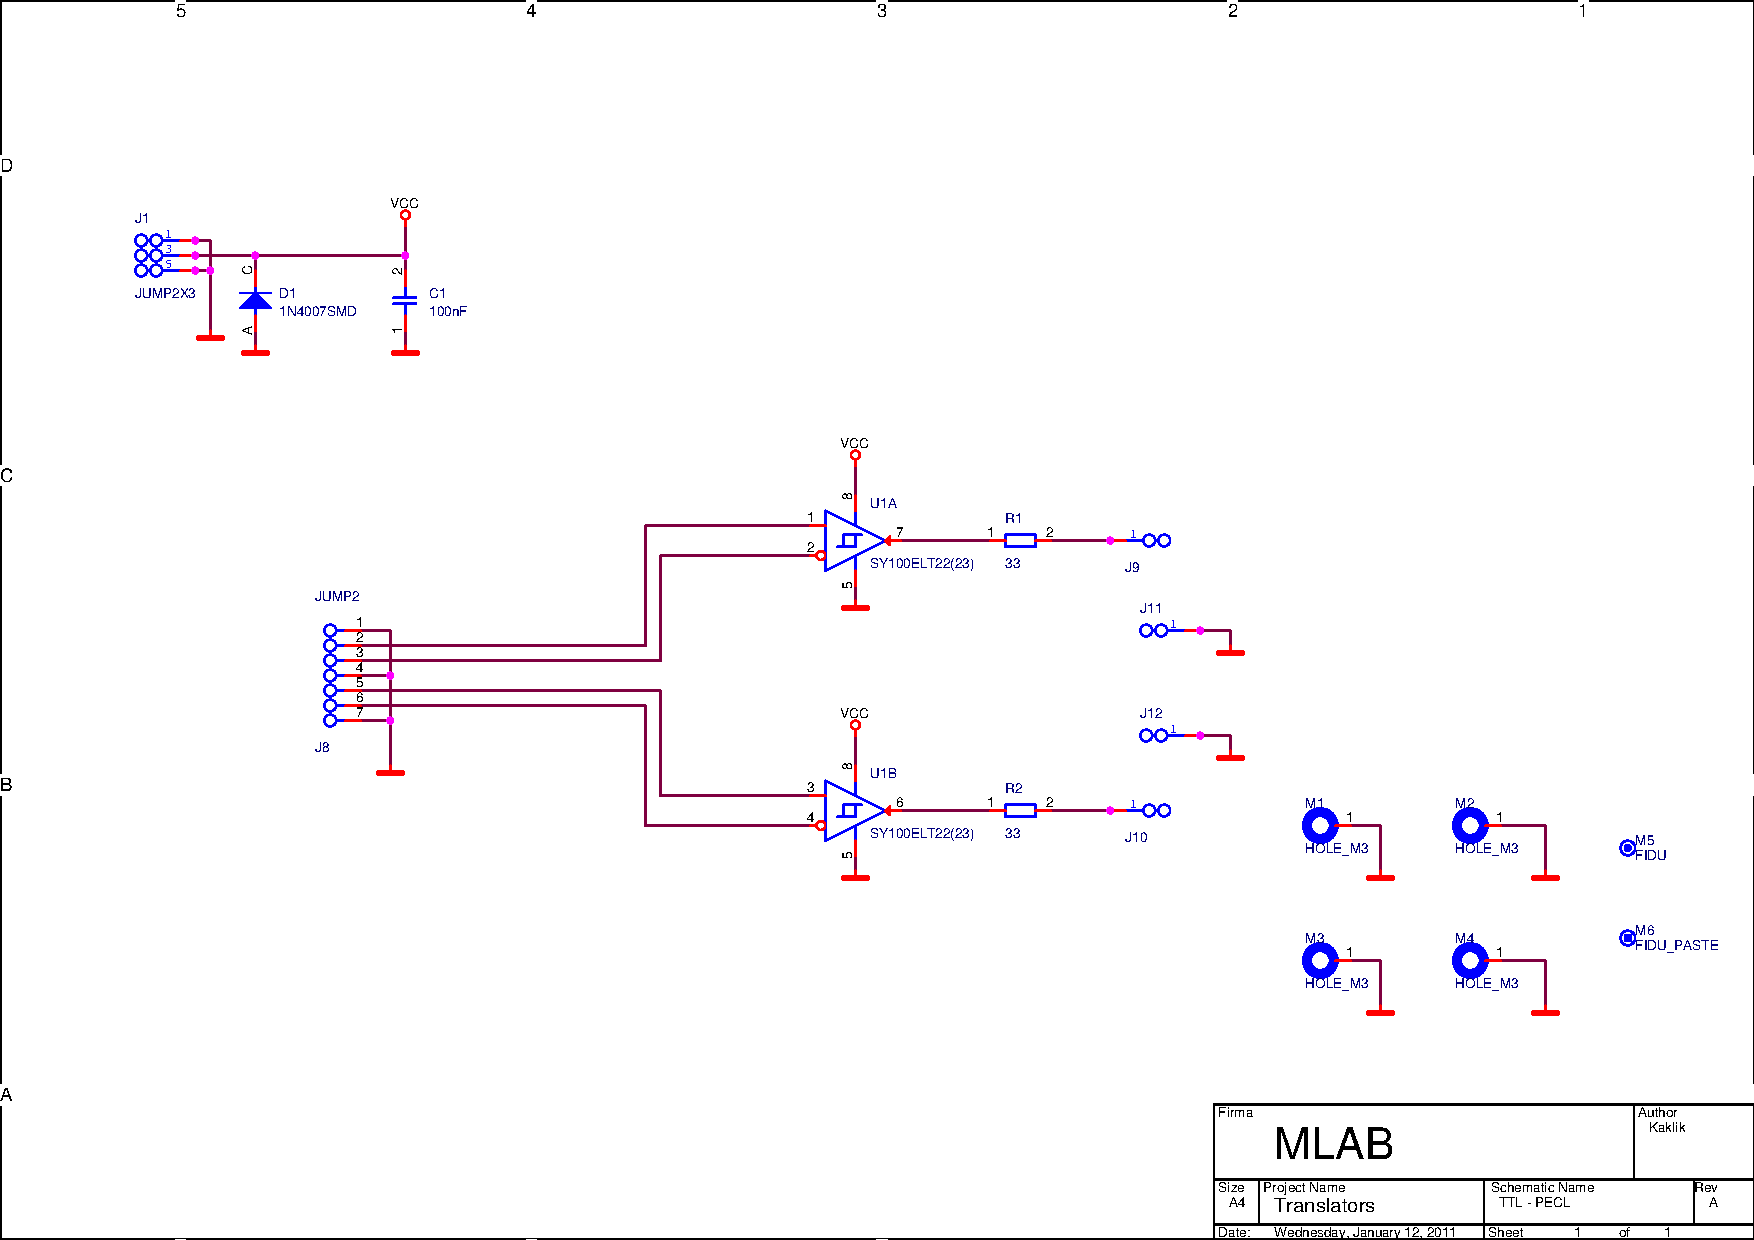
\includegraphics[trim = 5mm 50mm 80mm 15mm, clip, width=15cm]{../../SCH/ttlpecl.pdf}
\end{figure}

\section{Výroba a testování}

\subsection{Osazení}

\subsection{Ověření funkce}

\section{Použití modulu}

\subsubsection{Napájení}

Napájecí napětí modulu by mělo odpovídat napájecímu napětí související
logiky. A je 3,3V pro LVPECL a LVTTL a +5V pro PECL a TTL logiku. Je ale silně doporučeno moduly používat pouze s napájecím napětím 3,3 V.  

Pozor! V případě použití obvodu SY100ELT23L (Převod LVPECL na LVTTL) je
maximální dovolené napájecí napětí pouze 3,6V! Při jeho překročení může dojít
ke zničení modulu.

\end{document}